
%https://gateoverflow.in/118748/gate-cse-2017-set-1-question-54?show=118959#a118959
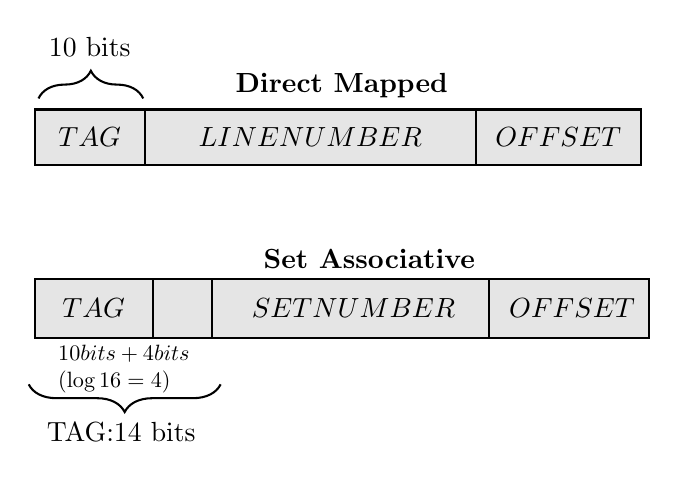
\begin{tikzpicture}[line width=.75pt]

\begin{scope}[scale=0.7]
  \draw[fill=gray!20] (0,0)node[xshift=0.7cm,yshift=1.5cm]{\text{10 bits}} rectangle(2,1);
  \draw[fill=gray!20] (2,0)node[xshift=2.5cm,yshift=1cm]{\textbf{\text{Direct Mapped}}}rectangle(8,1);
  \draw[fill=gray!20] (8,0)node[below]{}rectangle (11,1);
 
  \path (1,.5)node{$\text{TAG}$};
  \path (5,.5)node{$\text{LINE NUMBER}$};
  \path (9.5,.5)node{$\text{OFFSET}$};
  \draw [decorate,decoration={brace,amplitude=10pt,mirror,raise=4pt},xshift=2pt,rotate=180]
(-1.9,-1) -- (0,-1) ;
\end{scope}

\begin{scope}[yshift=-2.2cm,scale=0.75]
  \draw[fill=gray!20] (0,0)node[xshift=1.1cm,yshift=-0.4cm, text width=2cm,scale=0.8]{$\text{10 bits + 4 bits}$  $(\log 16 = 4)$} rectangle(2,1);
  \draw[fill=gray!20] (2,0)node[below]{} rectangle(3,1);
  \draw[fill=gray!20] (3,0)node[xshift=2cm,yshift=1cm]{\textbf{\text{Set Associative}}}rectangle(7.7,1);
  \draw[fill=gray!20] (7.7,0)node[below]{}rectangle (10.4,1);
 
  \path (1,.5)node{$\text{TAG}$};
  \path (5.4,.5)node{$\text{SET NUMBER}$};
  \path (9.1,.5)node{$\text{OFFSET}$};
  \node[xshift=1.1cm,yshift=-1.2cm]{TAG:14 bits};
  
  \draw [decorate,decoration={brace,amplitude=10pt,mirror,raise=4pt},xshift=0pt]
(-0.1,-0.6) -- (3.15,-0.6) ;
\end{scope}

\end{tikzpicture}
